\documentclass{article}
\usepackage{graphicx}
\usepackage[margin=1.5cm]{geometry}
\usepackage{amsmath}

\begin{document}

\title{Monday Reading Assessment: Unit 4, Forces}
\author{Prof. Jordan C. Hanson}

\maketitle

\section{Chapter 4 - Forces}

\begin{enumerate}
\item A rock of mass $m$ is thrown straight up. The net external force on the rock is
\begin{itemize}
\item A: $-mg$ on the way up, 0 at the top, and $-mg$ on the way down.
\item B: $-mg$ on the way up, $-mg$ at the top, and $-mg$ on the way down.
\item C: $+mg$ on the way up, $+mg$ at the top, and $+mg$ on the way down.
\item D: $+mg$ on the way up, 0 at the top, and $+mg$ on the way down.
\end{itemize}
\item A spring exerts a force $\vec{s} = -k \Delta\vec{x}$.  The displacement $\Delta\vec{x}$ is the amount the spring is stretched, and $k$ is a constant with units of Newtons per meter.  If a spring with $k = 50.0$ N/m is stretched by 10 cm, what is the force $\vec{s}$?
\begin{itemize}
\item A: -500 N
\item B: 500 N
\item C: -5 N
\item D: 5 N
\end{itemize}
\item 
\begin{figure}[ht]
\centering
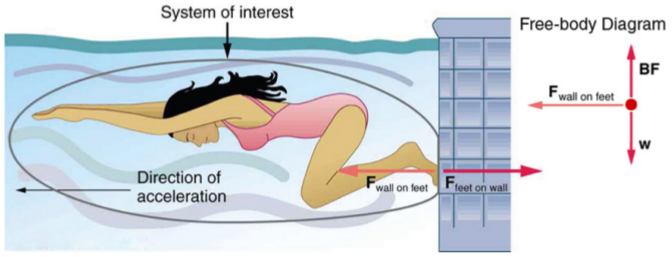
\includegraphics[width=0.6\textwidth]{wall.png}
\caption{\label{fig:wall} A woman pushes off of a wall underwater in a pool.}
\end{figure}
According to Fig. \ref{fig:wall}, a woman experiences a force by the wall on herself.  Her weight force $w$ is balanced by the buoyant force $BF$.  a) If the wall exerts a force of 100 N, and her mass is 50 kg, what is her acceleration?
\end{enumerate}

\end{document}
